
%%%%%%%%%%
\subsection{Principle of detection}
\label{sec:detection_principle}

The current detectors of gravitational waves are based on laser interferometry techniques.
They are based on the Michelson interferometer which consists in separating a laser beam towards two orthogonal arms of a given distance each, with mirors at their end, and recombine the separated laser at the output of the interferometer (figure \ref{fig:michelson}).
An interference pattern is created at the ouptput depending on the optical path length traveled by each laser beam.
This is exploited in gravitational waves detection: if the interferometer is locked and most source of noises are monitored and under control, the interference pattern at the output of the interferometer should not change since the length of the arms is constant.
Consider now the passing of a gravitational wave through the interferometer, with a propagation direction parallel to one of the arm of the interferometer.
This arm will be blind to the gravitational wave because it has no effect along its propagation axis but the other arm however is orthogonal to it, meaning that the proper distance between the beam splitter (BS) and the mirror of this arm will be subject to the proper distance oscillation caused by the wave.
The optical path length of the laser in this arm will be directly impacted and this will cause a shift in the phase difference of the lasers at the output of the interferometer and thus in the interference pattern.
For an interferometer locked in dark fringes mode (destructive interference and so no light at the output of the detector) the wave will cause it to stray away from the dark fringes conditions and a sensitive-enough photodiode can detect the light that pass through.

The quantity measured is called detector strain and is related to the displacement of the mirror by:
\begin{equation}
  h = \frac{\Delta L}{L_0}
\end{equation}
where $\Delta L = L_1-L_2$ is the length difference between the two arms of the interferometer and $L_0 = \textrm{\SI{3}{km}} (\textrm{\SI{4}{km}})$ for Virgo (LIGOs) is the arms length at rest.
This strain is dimensionless and varies with time, it is usually called ``h of t'' and written $h(t)$.
Calibration techniques have been developped to provide a precise measure of $h(t)$:
\begin{itemize}
\item The photon calibrator \cite{pcal} (Pcal) uses the radiation pressure of a laser beam to displace the end mirror of the interferometer.
  This was the reference technique for the calibration during O3.
\item The Newtonian calibrator \cite{ncal1,ncal2} (Ncal) is a newly developped calibration technique for the Virgo detector.
  Its principle is to induce a displacement of the end mirror using a varying gravitational field produced by rotating masses.
  It has the benefit of not needing an access window to the mirror as the gravitational force acts through matter.
\end{itemize}
\cite{strain_reconstruction} gives an overview of the calibration and reconstruction of the strain for Virgo during O3.
%
\begin{figure}
  \centering
  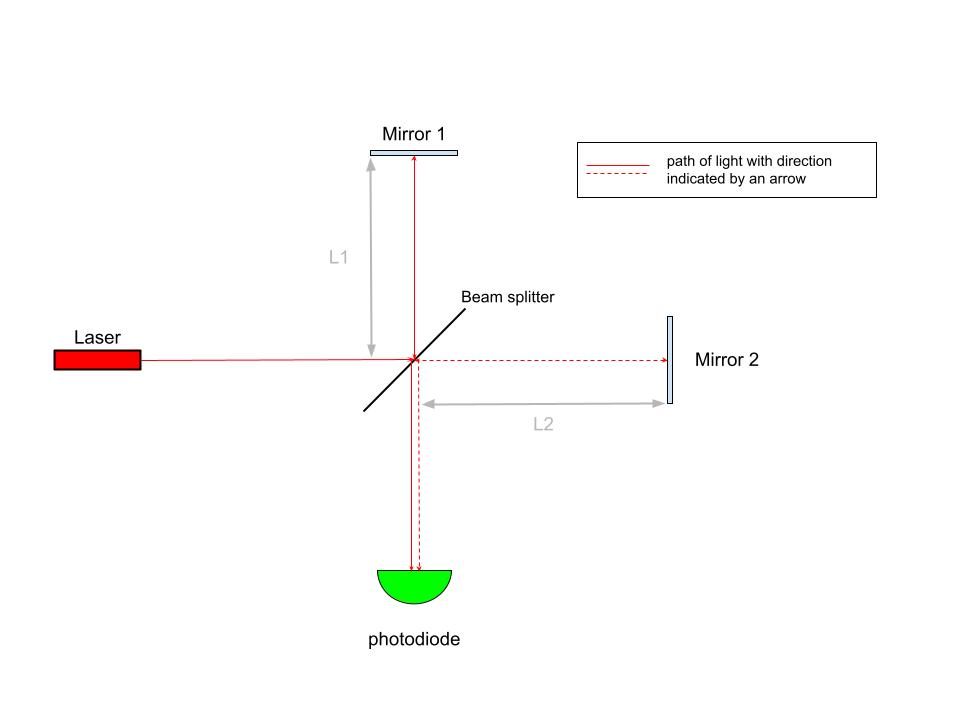
\includegraphics[width=0.5\linewidth]{sectionDetection/michelson.jpg}
  \caption{Schematic view of a simple Michelson interferometer}
  \label{fig:michelson}
\end{figure}


%%%%%%%%%%
\subsection{Detectors' description}
\label{sec:detector}

The LIGO and Virgo interferometers are of course much more complex than a simple Michelson interferometer.
A simplified version of the Virgo optical layout is shown in figure \ref{fig:virgo_layout}.
An interested reader may find the full details of the interferometer in \cite{advanced_virgo,virgo_tech_report} and the various papers cited in this section.
We are only going to highlight the main parts to describe figure \ref{fig:virgo_layout}:
\begin{itemize}
\item A 200W laser,
\item Fabry-Perot cavities created in each arm with the input mirrors (IM) and end mirrors (EM).
  These cavities, by making the laser beam reflect back and forth, increase the  optical path length by a factor close to 290 (for Virgo) making the detector very sensitive.
  The mirrors are made of fused silica (Suprasil 3002 for the IM and Suprasil 312 for the EM) coated with Ti doped Ta$_2$O$_5$.
  They are suspended by four silica fibers to a steel structure in a double pendulum fashion, which is in turn suspended to the super attenuator consisting of a chain of seismic filters.
\item Compensation Plates (CP) to stem thermal effects and a Pick-Off Plate (POP) to retrieve a fraction of the beam for monitoring.
\item A Power Recycling Mirror (PRM) to increase the laser power in the amrs of the interferometer and reduce the uncertainty on photon counting, and a Signal Recycling Mirror (SRM) for a better sensitivity \cite{recycling1,recycling2}.
\item An input and output mode cleaner (IMC/OMC) for a better beam quality.
\item A photodiode at the output (B1).
\end{itemize}
All of these components are placed in vacuum.
%
\begin{figure}
  \centering
  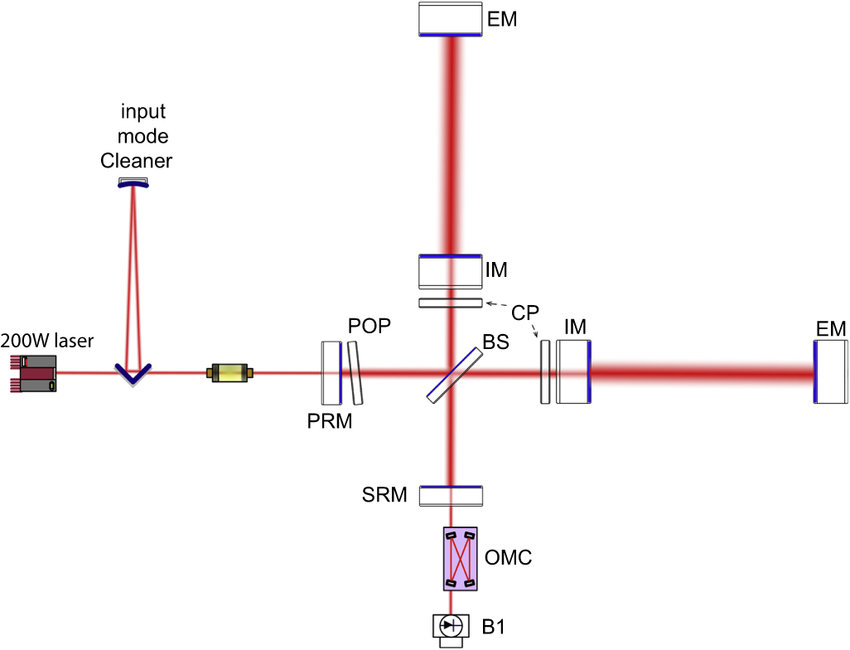
\includegraphics[width=0.5\linewidth]{sectionDetection/simple_virgo_layout.png}
  \caption{Simplified Virgo optical layout from \cite{advanced_virgo} described in the text.}
  \label{fig:virgo_layout}
\end{figure}
%

The response of the detector to an incoming gravitational wave can be modelled by its antenna patterns.
They correspond to the response as a function of the direction of the wave with respect to the orientation of the detector such that
\begin{equation}
  h = F_+ h_+ + F_\times h_\times
\end{equation}
with \cite{antenna_patterns}
\begin{align}
  F_+ &= -\frac{1}{2}(1+\cos^2\theta) \cos 2\phi \cos 2\psi - \cos \theta \sin 2\phi \sin 2 \psi\\
  F_\times &= \frac{1}{2}(1+\cos^2\theta) \cos 2\phi \sin 2\psi - \cos \theta \sin 2\phi \cos 2 \psi
\end{align}
the antenna response pattern of the detector to the plus and cross polarizations respectively with $\theta$ and $\phi$ the sky location angles of the source and $\psi$ the polarization angle.
Figure \ref{fig:antenna_pattern} shows these patterns for a polarization angle of 0.
We see that the best-case scenario is a wave propagating along the axis orthogonal to both arms of the interferometer.
%
\begin{figure}
  \centering
  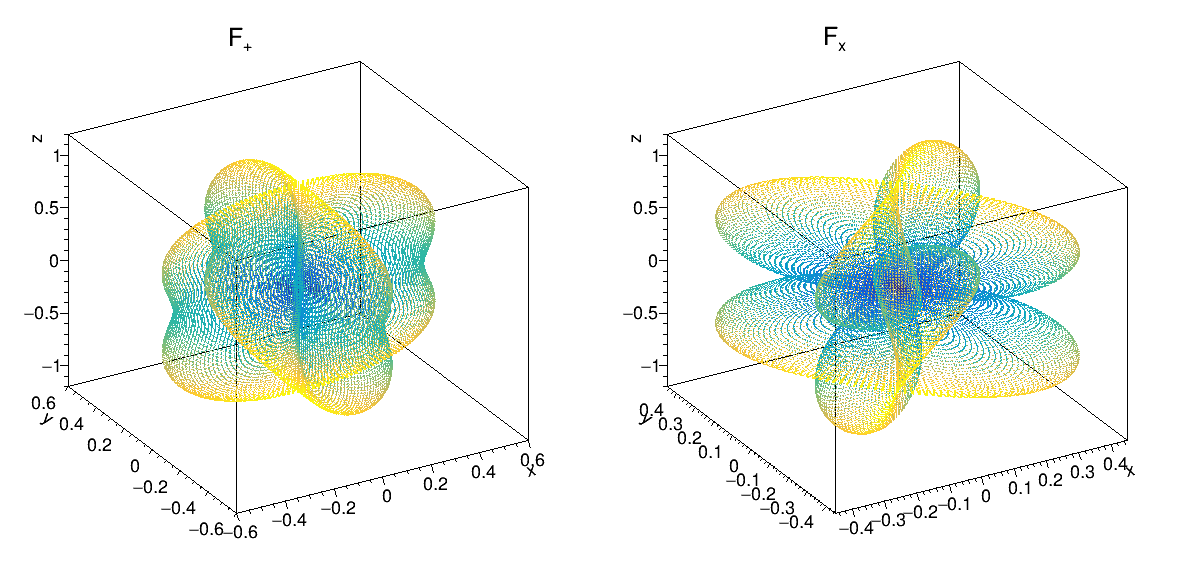
\includegraphics[width=0.5\linewidth]{sectionDetection/antenna.png}
  \caption{\textcolor{red}{à faire}}
  \label{fig:antenna_pattern}
\end{figure}
%

The high sensitivity of these intruments makes them extremely sensible to numerous sources of noise on which the reader may find more details in references \cite{ligo_characterization} to \cite{prospects}.
The sensitivity of a detector is characterized by its noise power spectral density (PSD).
Figures \ref{fig:ligo_sensitivity} and \ref{fig:virgo_sensitivity} show the noise budget of the LIGO and Virgo detectors.

Several quantities are used to quantify the sensitivity of a detector with a single value \cite{findchirp,distances,one_ifo}:
\begin{itemize}
\item The horizon distance is defined for a given type of source and a given signal-to-noise ratio (SNR) threshold $\rho$ (detailled in section \ref{section:mbta}).
  It is the effective distance (eq. \ref{eq:effective_distance}) for which this type of source would give an expected SNR of $\rho$, in other words it is the maximum distance at which we could detect this source above threshold.
  The horizon distance is given by \cite{findchirp} (Appendix D)
  \begin{equation}
    D_{\textrm{horizon}} = \frac{1}{\rho} \frac{(GM_c)^{5/6}}{\pi^{2/3}c^{3/2}} \frac{\msun^{5/3}}{\textrm{\SI{1}{Mpc}}} \sqrt{\left(\frac{5}{6}\right) \int_{0}^{\infty}\frac{f^{-7/3}}{S_n(f)}df}
    \label{eq:horizon}
  \end{equation}
  with $S_n(f)$ the noise PSD.
  In practice the integration is actually done from $f_{\textrm{low}}$, the frequency at which the signals enters the interferometer bandwidth, and $f_{\textrm{ISCO}}$ the frequency of the binary at its innermost stable circular orbit defined as
\begin{equation}
  f_{\textrm{ISCO}} = \frac{c^3}{6\sqrt{6}\pi G M_{\textrm{tot}}}
\end{equation}
The horizon distance is typically computed for a BNS system of $1.4+1.4$ \msun and an SNR threshold $\rho=8$.

\item The redshifted comoving volume $V_z$ expressed per unit of time \cite{distances}
  \begin{equation}
    V_z = \frac{ \int_{D<D_{\textrm{horizon}}} \frac{D^2}{1+z(D)} dD \hspace{1pt} d\Omega \hspace{2pt} \sin i \hspace{2pt} di \hspace{2pt} d\psi}{\int \sin i \hspace{2pt} di \hspace{2pt} d\psi}
  \end{equation}
  with $D$ the comoving distance to the source, $\Omega$ is the solid angle on the sky, $i$ the inclination of the system and $\psi$ the orientation of the source.

\item The euclidean volume with the same volume as the redshifted volume multiplied by the observing time is called ``volume-time'' (VT) and is proportional to the number of detection.
  Indeed for a population of $N_{\textrm{source}}$ sources uniformely distributed within a sphere of radius $D_{\textrm{horizon}}$, only a smaller number ,$N_{\textrm{det}}$, of them will be detectable since some will have $D_{\textrm{eff}}>D_{\textrm{horizon}}$.
  In other words for $N_{\textrm{det}}$ detections above a SNR threshold over a given time, the VT is the observing time multiplied by the volume of the sphere that would contain as many detectable sources above threshold assuming a uniform source distribution.
  
\item The range is more commonly used to  refer to a detector's sensitivity.
  It is the radius of a sphere with volume equal to $V_z$, i.e.
  \begin{equation}
    \frac{4}{3} \pi \times \textrm{range}^3 = V_z
  \end{equation}
  Since the horizon distance is computed for a given type of source and an SNR threshold, it is also the case for all other quantities described here.
  The range is typically computed for a $1.4 + 1.4$ \msun BNS system and an SNR threshold of 8 and we talk of BNS range.
  Figure \ref{fig:sensitivity_comparison} shows a comparison of the BNS ranges of the LIGOs and Virgo detectors during O2 and O3 as well as their PSDs.
\end{itemize}
A comparison of the target sensitivities of the LIGO, Virgo and KAGRA detectors is shown in figure \ref{fig:design_sensitivities}.


\begin{figure}
  \centering
  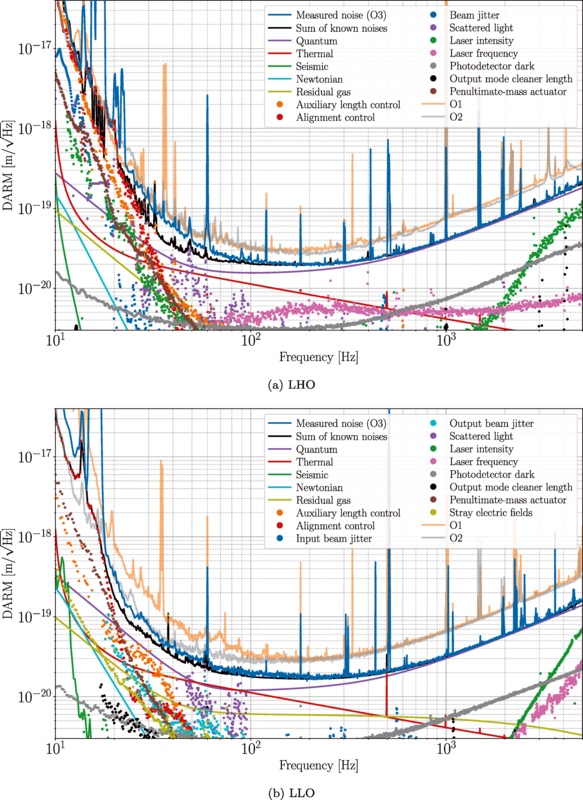
\includegraphics[width=0.5\linewidth]{sectionDetection/ligo_sensitivity.png}
  \caption{Noise budget of the LIGO Livingstong and Hanford observatories during O3 from \cite{ligo_sensitivity}.}
  \label{fig:ligo_sensitivity}
\end{figure}


\begin{figure}
  \centering
  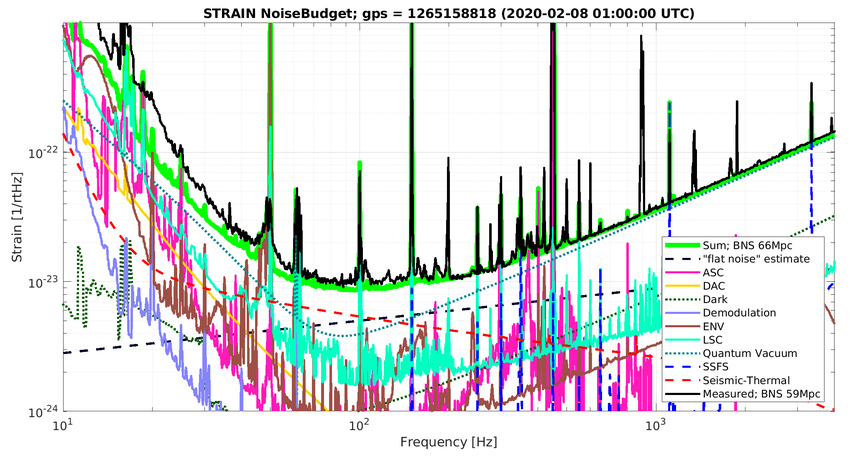
\includegraphics[width=0.5\linewidth]{sectionDetection/virgo_noise.png}
  \caption{Noise budget of the Virgo detector from \cite{virgo_characterization}.}
  \label{fig:virgo_sensitivity}
\end{figure}


\begin{figure}
  \centering
  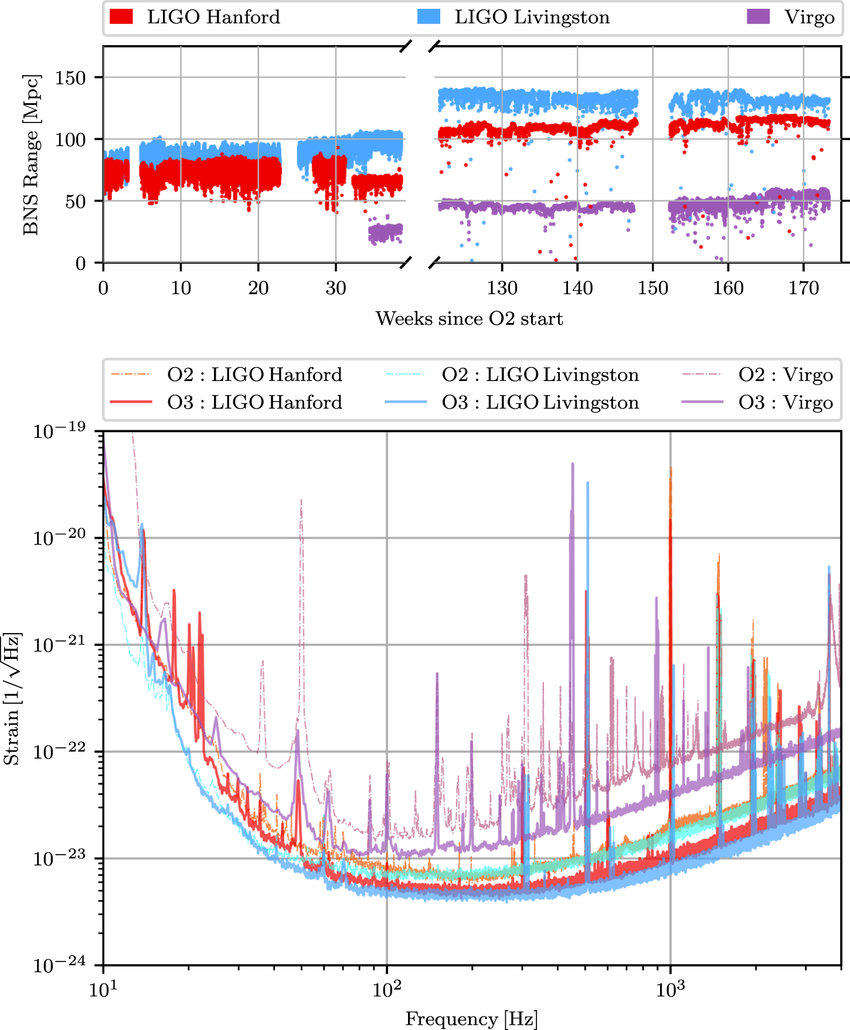
\includegraphics[width=0.5\linewidth]{sectionDetection/sensitivity_comparison.png}
  \caption{O3 and O2 sensitivity comparison of the LIGO and Virgo detectors from \cite{ligo_characterization}.}
  \label{fig:sensitivity_comparison}
\end{figure}


\begin{figure}
  \centering
  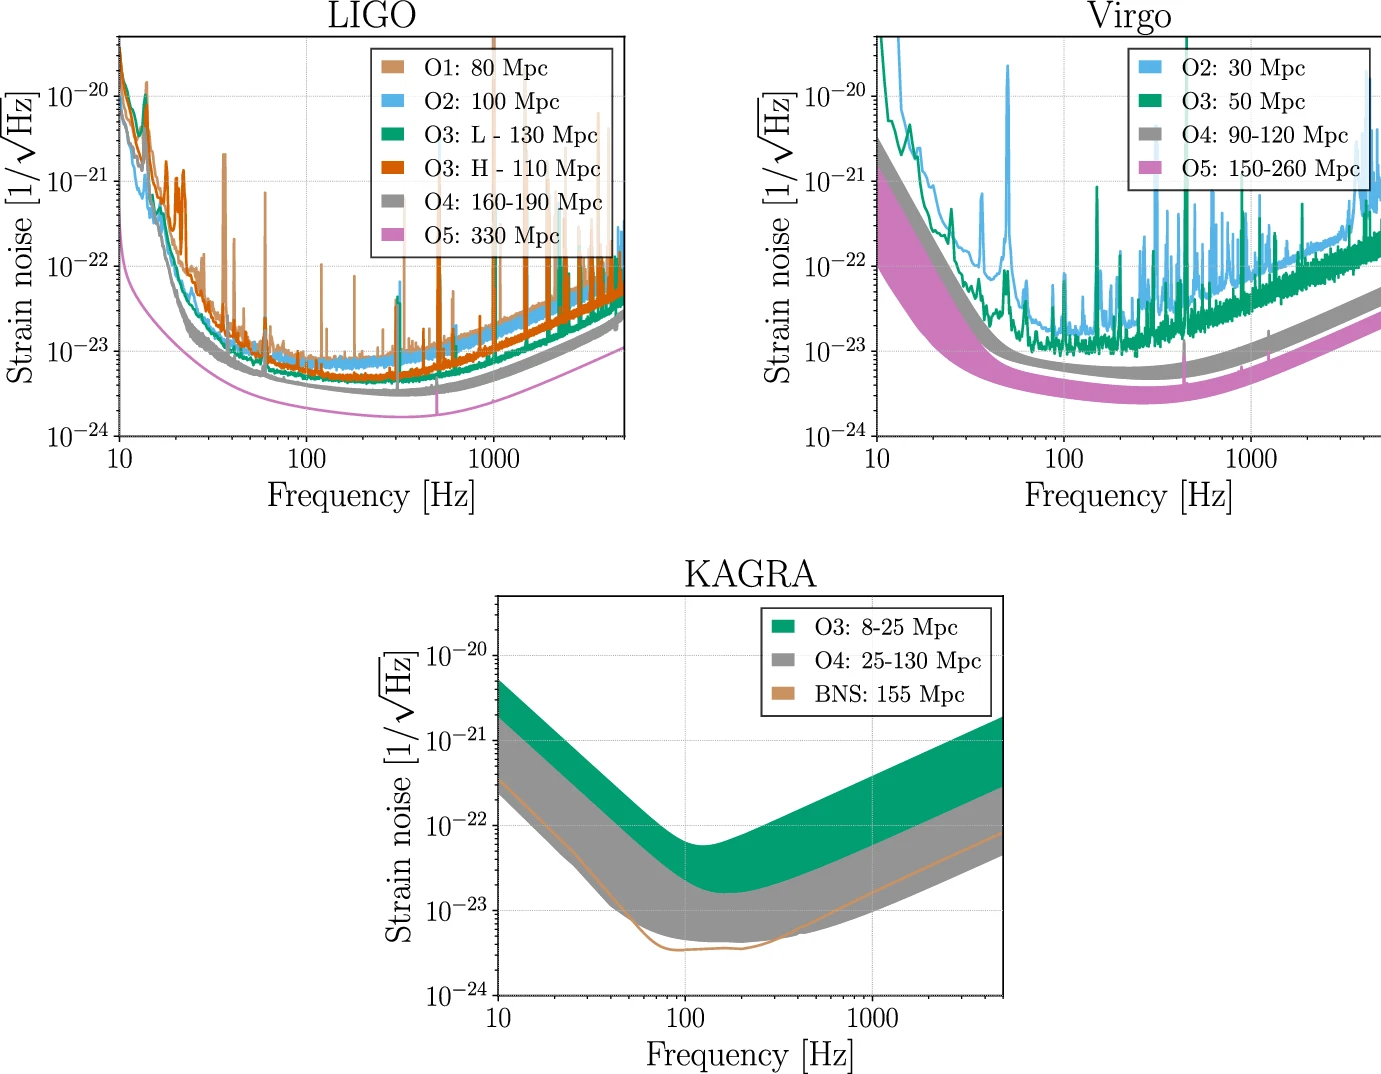
\includegraphics[width=0.5\linewidth]{sectionDetection/design_sensitivities.png}
  \caption{Target sensitivities for the LIGO, Virgo and KAGRA detectors from \cite{prospects}.}
  \label{fig:design_sensitivities}
\end{figure}



%%%%%%%%%%
\clearpage \newpage
\subsection{Network of detectors and sky localization}
\label{sec:network}

We have on earth a total of four gravitational waves detector: LIGO Hanford (USA), LIGO Livingston (USA), Virgo (Italy) and KAGRA (Japan).
A fifth detector, GEO600 (Germany) is used mostly for the research and developpment of equipment destined to the other interferometers.
A LIGO India detector is planned for construction.
Figure \ref{fig:igwn} shows the network of interferometer on a map.
%
\begin{figure}
  \centering
  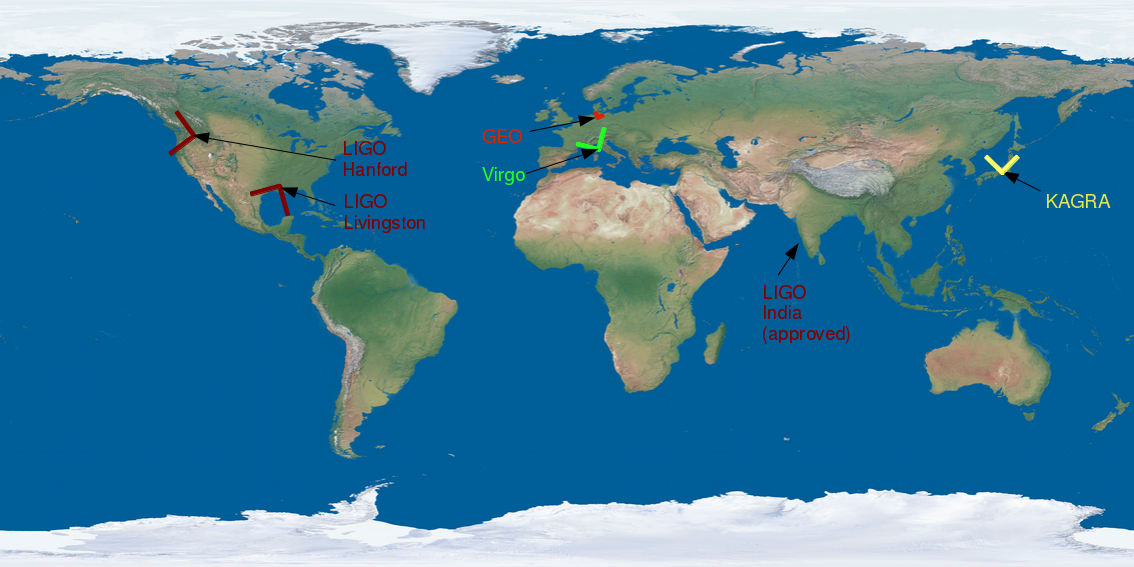
\includegraphics[width=0.5\linewidth]{sectionDetection/itf_network.png}
  \caption{The International Gravitational Wave Observatory Network (IGWN) map with orientation of the detectors. Taken from the \href{http://public.virgo-gw.eu/a-worldwide-network/}{Virgo website}.}
  \label{fig:igwn}
\end{figure}
%
There are multiple benefits in having several detectors:

By placing them at different location on earth with varying orientation the antenna patterns of the detectors complement each other allowing for a much better sky coverage than a single detector, thus increasing the chances of detection.

Another advantage is the possibility of searching for coincident signal in several detectors.
It is safe to assume the noise of the detectors are uncorrelated since it is only due to local factors and they are largely separated.
Therefore a significant noise event in one detector is unlikely to be associated to a significant noise event in antoher detector.
But in the case of an astrophysical signal, the waves travel through the earth and all detectors are susceptible to detect it and we expect to have a significant trigger at the same time (accounting for the time of flight of the waves).
This is a powerful criteria to discriminate astrophysical signals from noise.

A third benefit which is the product of the two previous consideration is the improved sky location of the source in case of detection with multiple detectors.
Given the SNR time series and the time delay between the detectors it is possible to triangulate the most likely location for the gravitational wave source.
Even the non-detection of a signal is a valuable information as it indicates that the source may be located in a direction to which the said detector is not sensitive.
The process of localization is illustrated in figure \ref{fig:localization} using GW170817 as an example.
From left to right and top to bottom: the antenna patterns of H1 and L1 give an information to what directions they are sensitive to.
The timing information allows to derive a line on the sky on which the source should be located.
Including the SNR information allows to derive a contour for the location.
Adding V1, which did not detect the signal gives an additional information.
By comparing the expected SNR as a function of the sky location to what was observed allows to constrain the contour and gives a refined measurement of the source location.

\begin{figure}
  %
  % 1
  \begin{minipage}{0.45\linewidth}
    \centering
    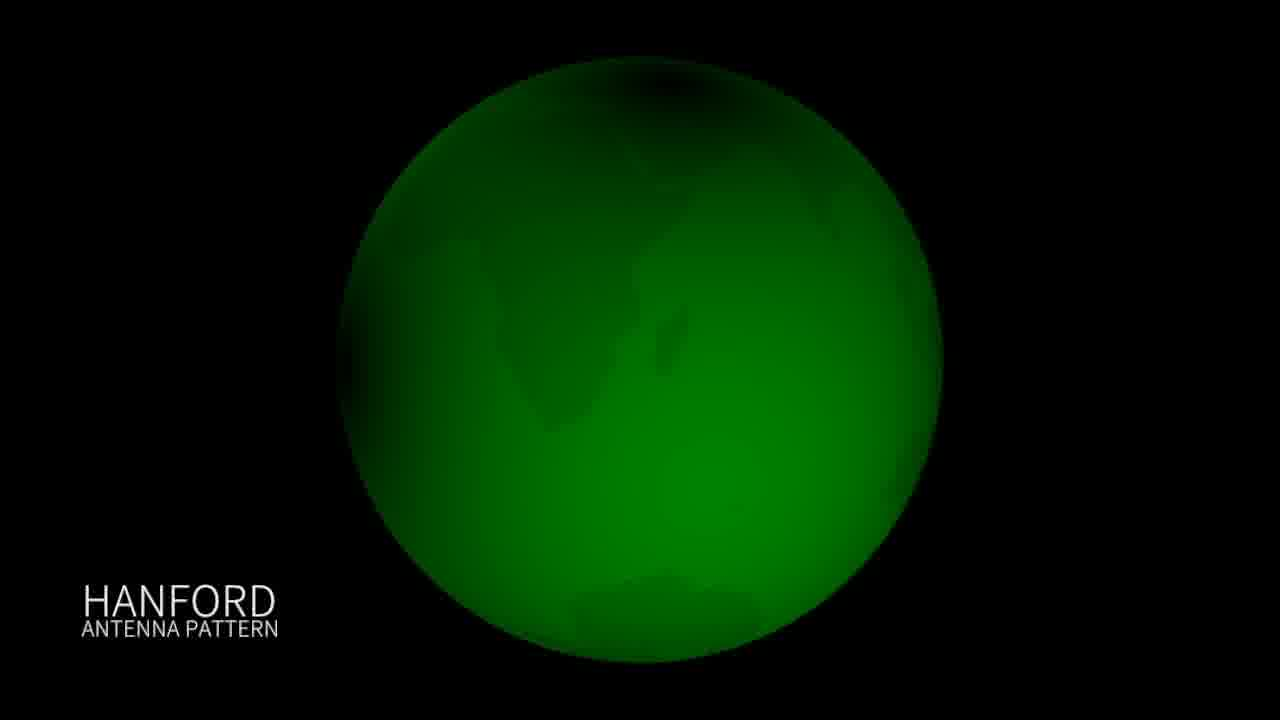
\includegraphics[width=\linewidth]{sectionDetection/antenna-patterns_LeoSinger/00012.jpg}
    %\captionof*{figure}{(a) LIGO Hanford antenna pattern, the dark areas are the less sensitive ones.}
  \end{minipage}
  %
  \hfill
  % 2
  \begin{minipage}{0.45\linewidth}
    \centering
    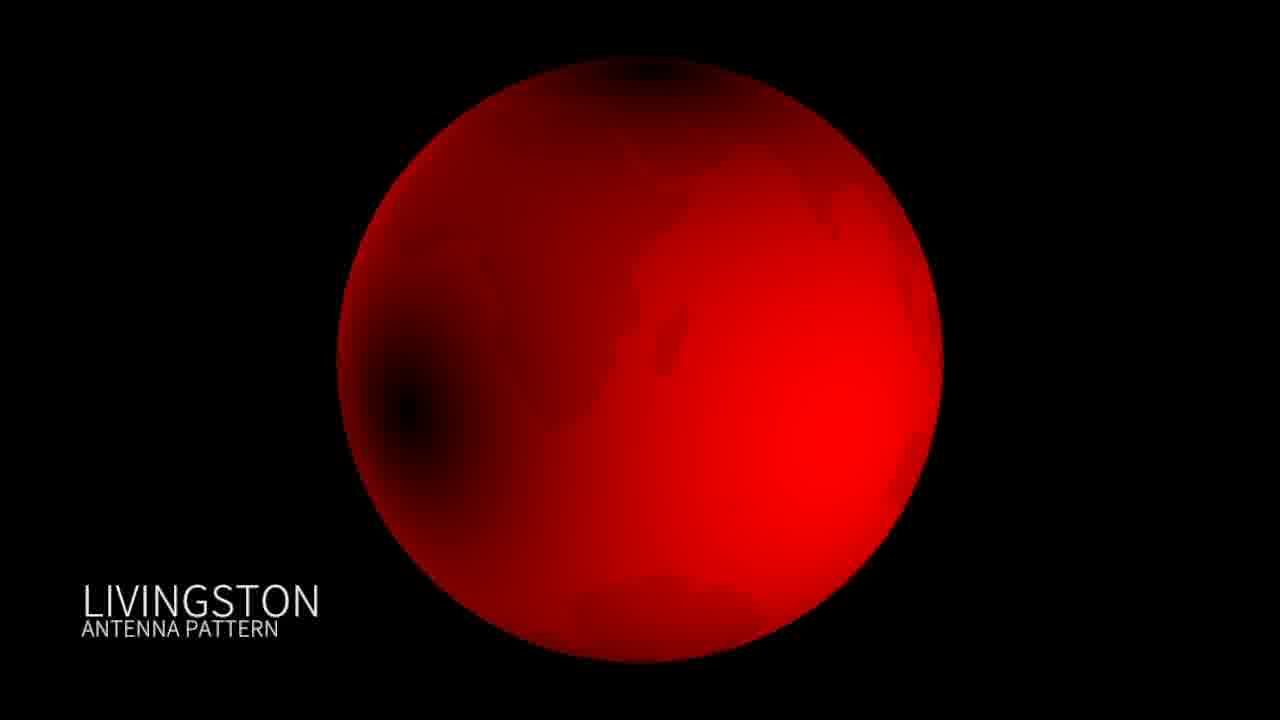
\includegraphics[width=\linewidth]{sectionDetection/antenna-patterns_LeoSinger/00118.jpg}
    %\captionof*{figure}{(b) LIGO Livingston antenna pattern, the dark areas are the less sensitive ones.}
  \end{minipage}
  %
  \hfill
  % 3
  \begin{minipage}{0.45\linewidth}
    \centering
    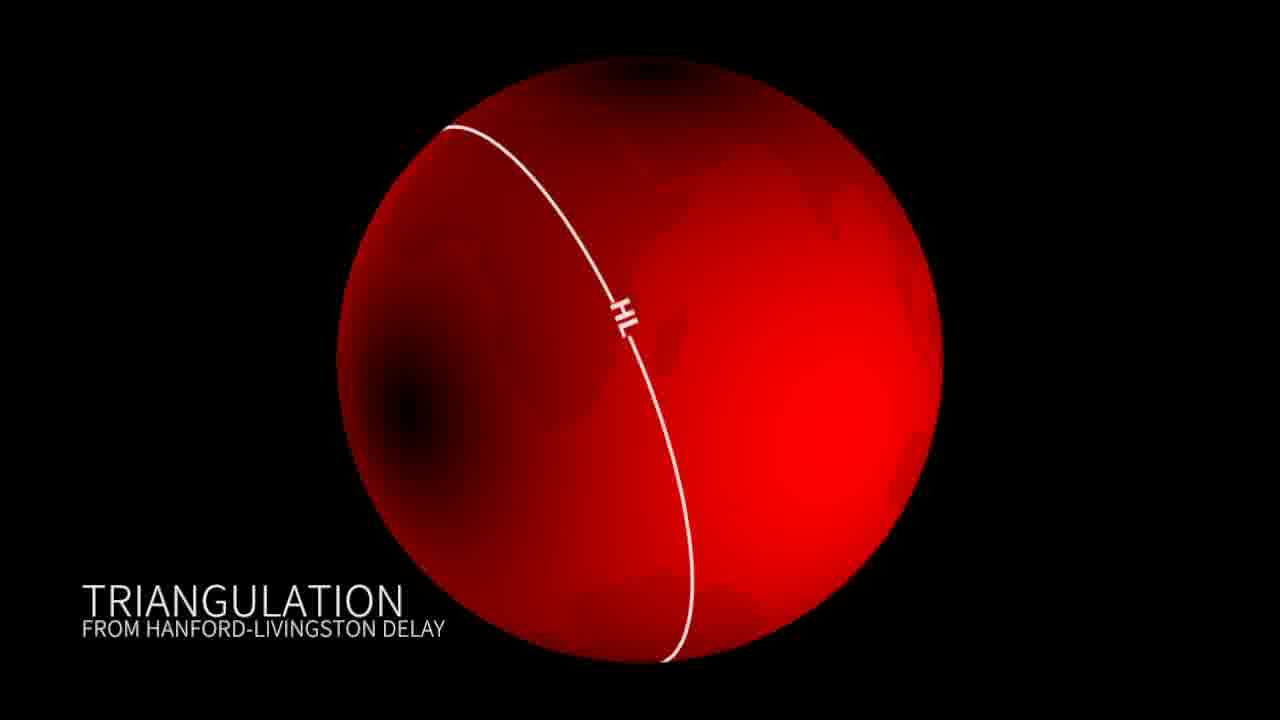
\includegraphics[width=\linewidth]{sectionDetection/antenna-patterns_LeoSinger/00227.jpg}
    %\captionof*{figure}{(c) Line of sight given by the timing information between H1 and L1.}
  \end{minipage}
  %
  \hfill
  % 4
  \begin{minipage}{0.45\linewidth}
    \centering
    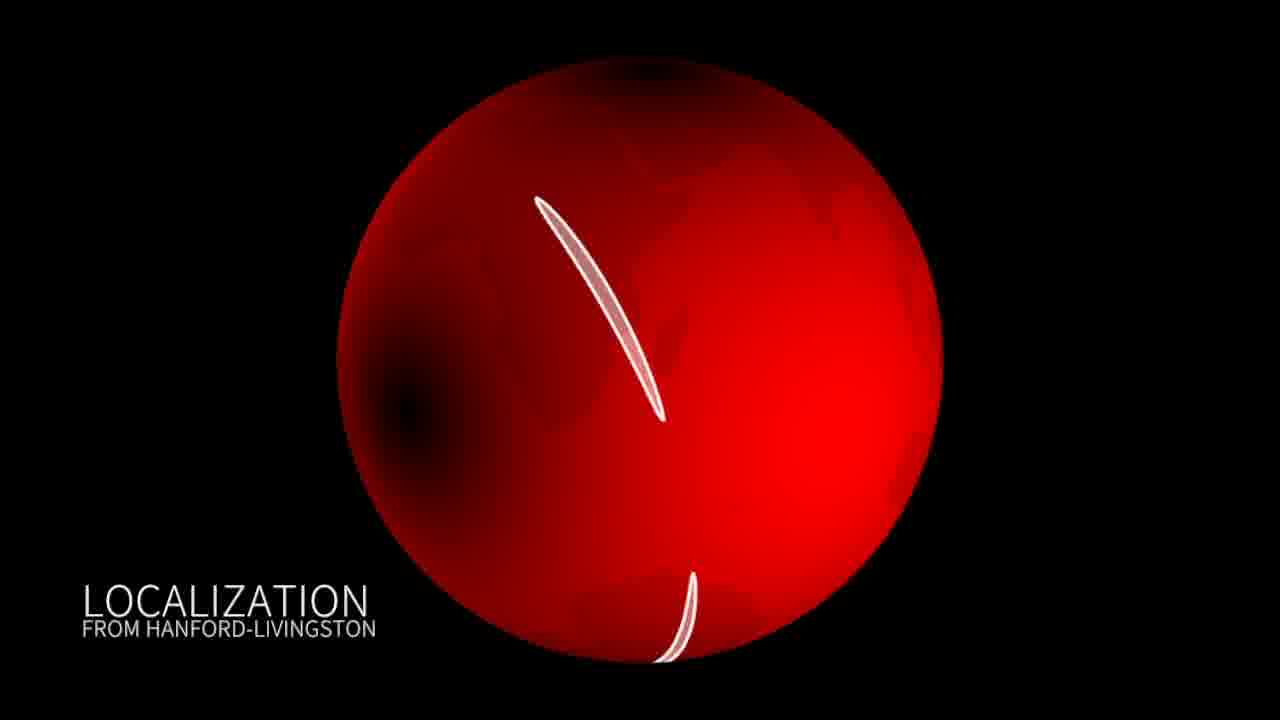
\includegraphics[width=\linewidth]{sectionDetection/antenna-patterns_LeoSinger/00318.jpg}
    %\captionof*{figure}{(d) Source localization contour obtained by accounting for the SNR in H1 and L1.}
  \end{minipage}
  %
  \hfill
  % 5
  \begin{minipage}{0.45\linewidth}
    \centering
    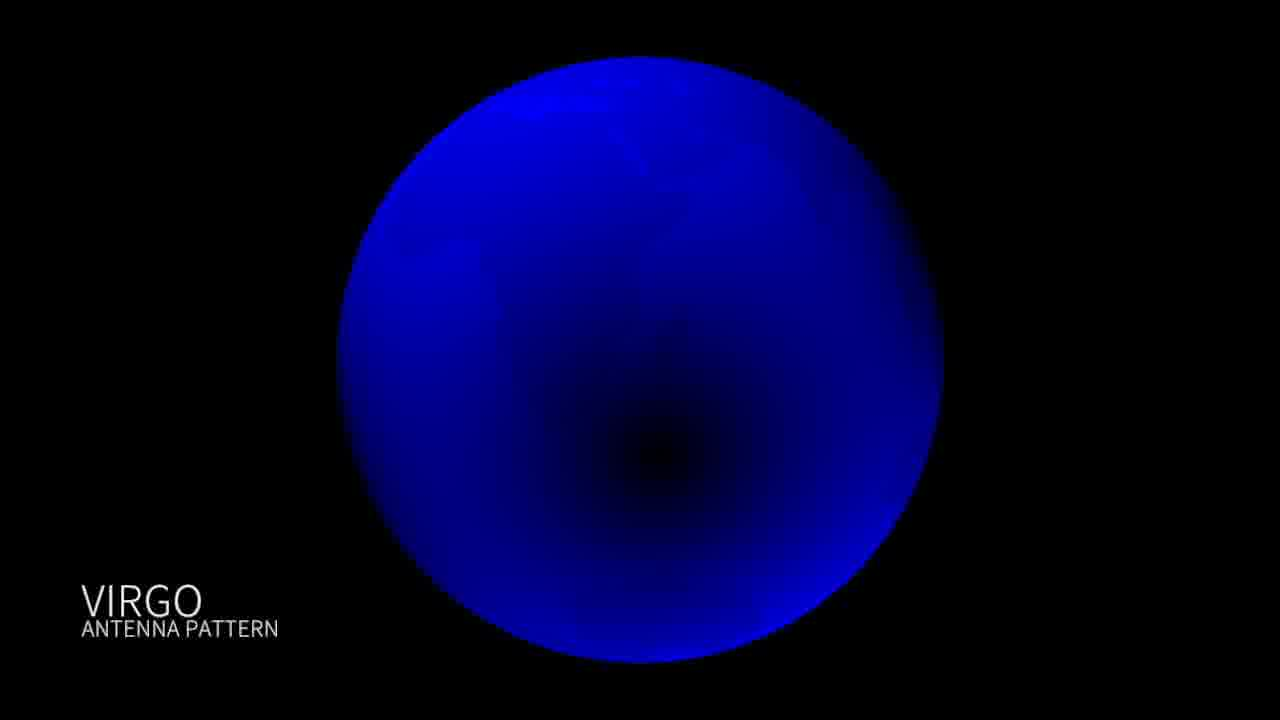
\includegraphics[width=\linewidth]{sectionDetection/antenna-patterns_LeoSinger/00418.jpg}
    %\captionof*{figure}{(e) Virgo antenna pattern, the dark areas are the less sensitive ones.}
  \end{minipage}
  %
  \hfill
  % 6
  \begin{minipage}{0.45\linewidth}
    \centering
    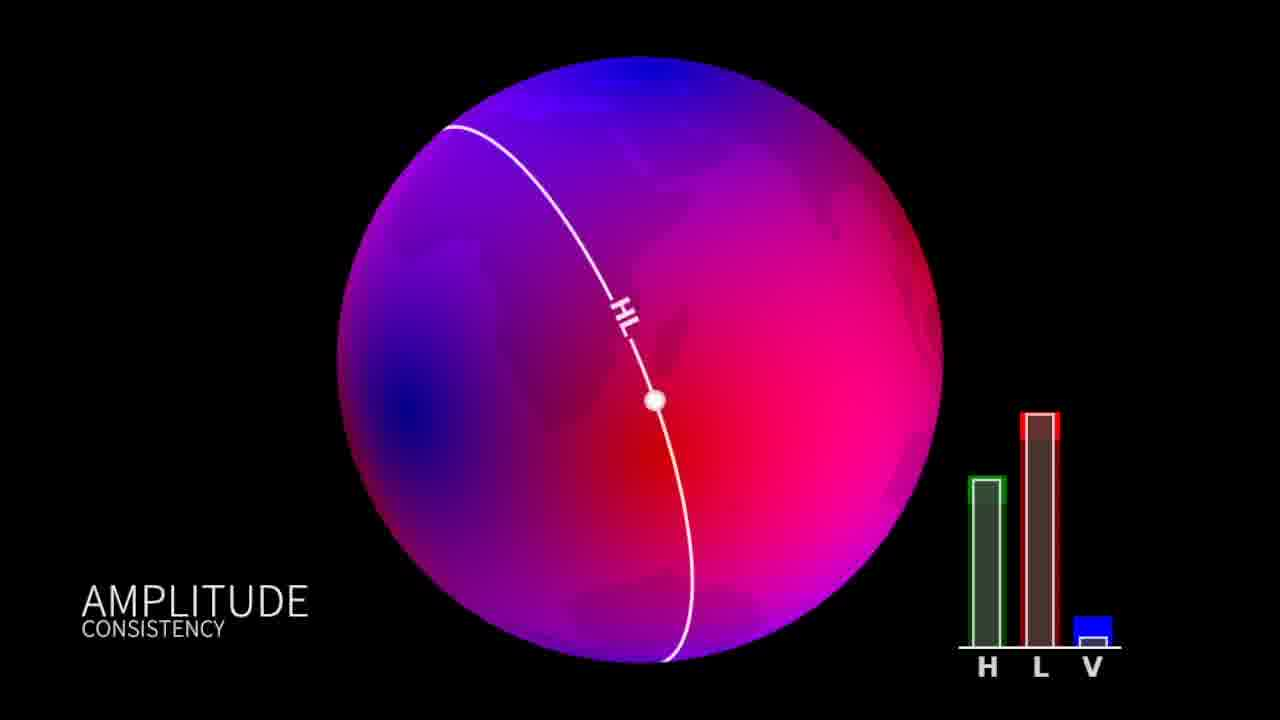
\includegraphics[width=\linewidth]{sectionDetection/antenna-patterns_LeoSinger/00552.jpg}
    %\captionof*{figure}{(f) Attempt at finding the source localization by estimating the expected SNRs int the three detectors.}
  \end{minipage}
  %
  \hfill
  % 7
  \begin{minipage}{0.45\linewidth}
    \centering
    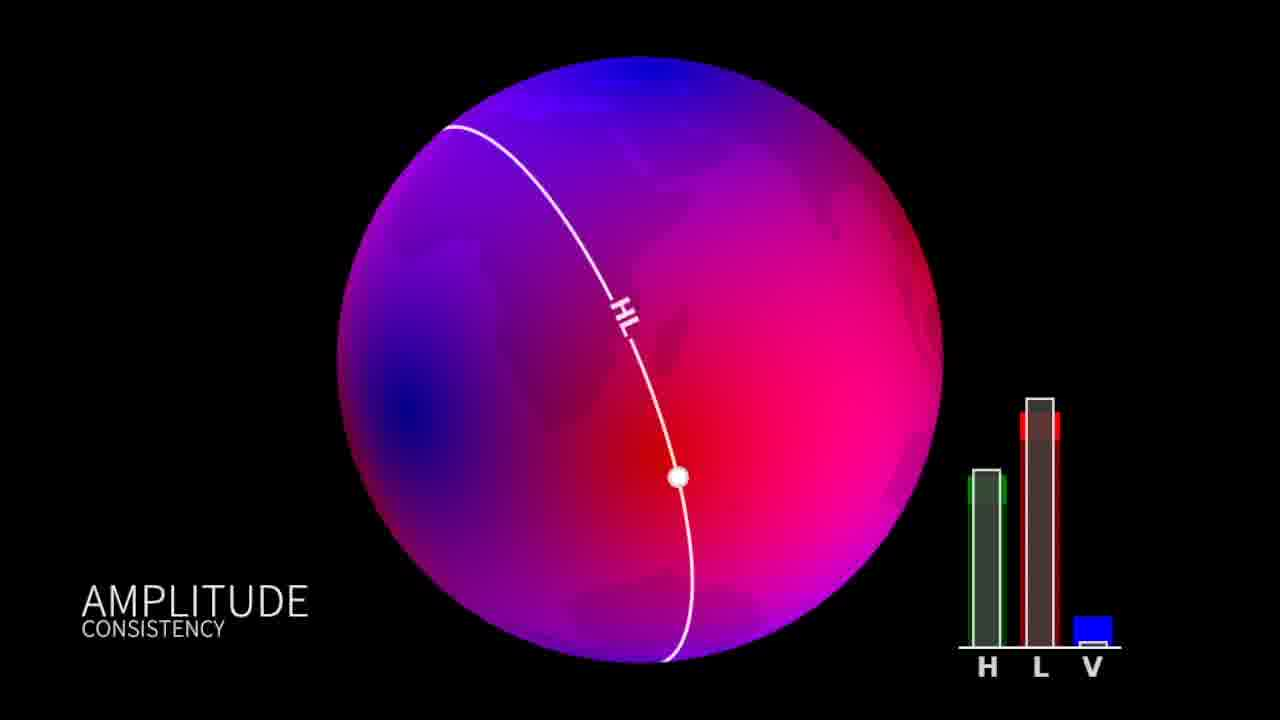
\includegraphics[width=\linewidth]{sectionDetection/antenna-patterns_LeoSinger/00559.jpg}
    %\captionof*{figure}{(g) Attempt at finding the source localization by estimating the expected SNRs int the three detectors.}
  \end{minipage}
  %
  \hfill
  % 8
  \begin{minipage}{0.45\linewidth}
    \centering
    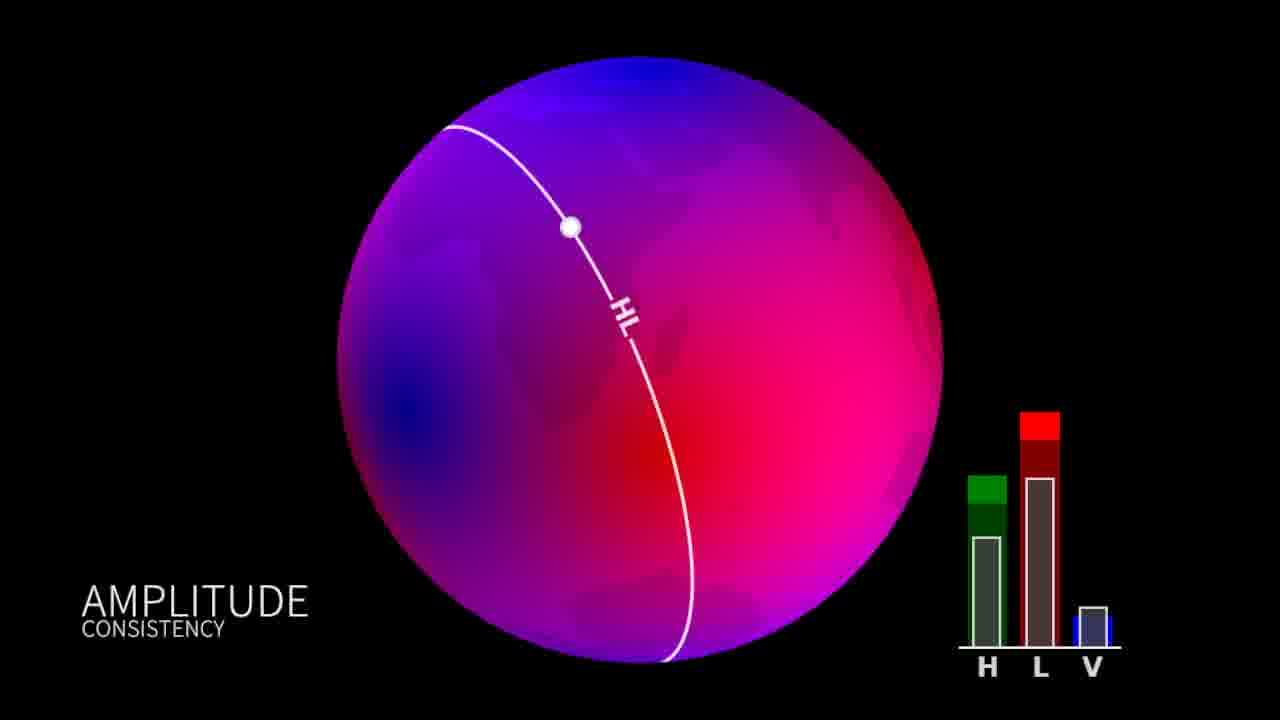
\includegraphics[width=\linewidth]{sectionDetection/antenna-patterns_LeoSinger/00584.jpg}
    %\captionof*{figure}{(h) Attempt at finding the source localization by estimating the expected SNRs int the three detectors.}
  \end{minipage}
  %
  \hfill
  % 9
  \centering
  \begin{minipage}{0.45\linewidth}
    \centering
    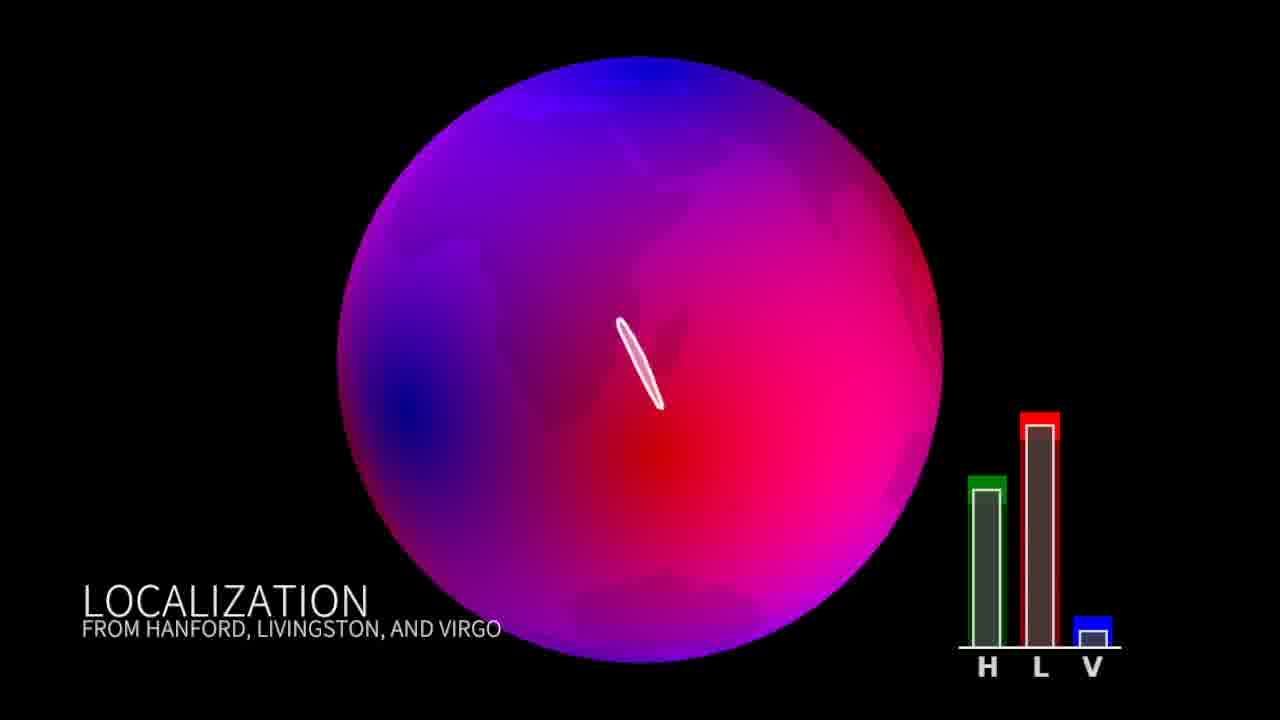
\includegraphics[width=\linewidth]{sectionDetection/antenna-patterns_LeoSinger/00900.jpg}
    %\captionof*{figure}{(i) Refined source localization contour obtained by including V1.}
  \end{minipage}
  %
  \hfill
  \caption{Illustration of the process of localizing the source for GW170817 made by Leo Singer (original format available at \url{https://dcc.ligo.org/LIGO-G1702012/public}). See the text for a description.}
  \label{fig:localization}
\end{figure}


%%%%%%%%%%
\subsection{Online alerts}
In the case of GW170817, one more information was available to localize the source: the electro-magnetic counterpart that was detected.
This joint observation allowed to pinpoint even more precisely the source location as shown by figure \ref{fig:gw170817_location}.
%
\begin{figure}
  \centering
  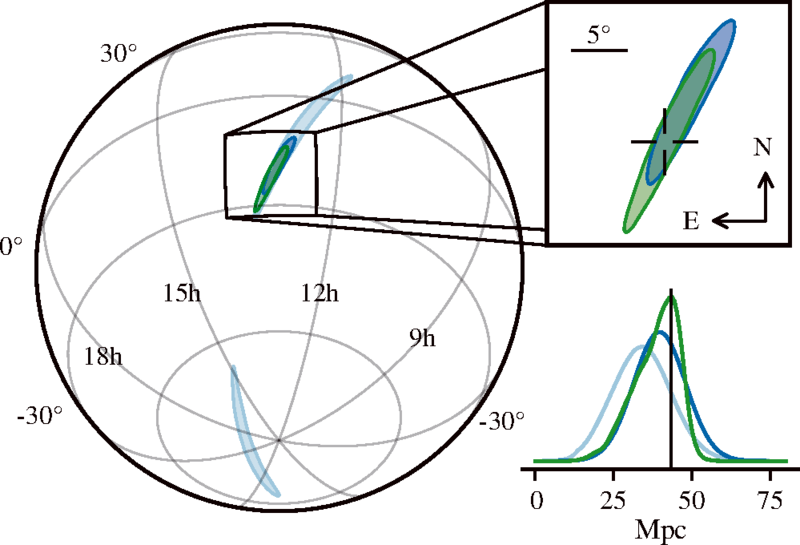
\includegraphics[width=0.5\linewidth]{sectionDetection/gw170817_location.png}
  \caption{Reconstructed sky location for GW170817 from \cite{gw170817}. The light blue area (190 deg$^2$) is computed by a fast-response algorithm using H1 and L1 only, the dark blue (31 deg$^2$) includes V1. The green contour (28 deg$^2$) includes the three detectors and is given by a code with higher latency. The reticle in the top right panel indicates the location for the galaxy identified as host and the bottom right panel shows the posterior luminosity distance distribution.}
  \label{fig:gw170817_location}
\end{figure}
%
It was made possible by the public alert system of the LVK collaboration and many observatories thoughout the world.
When a significant candidate is reported by at least one of the pipelines an alert is published online on the GraceDB website and a circular and notice are sent to any observer who requested it.
Candidates uploaded by search pipeline on GraceDB are called G-event and list some of the signal properties reported by the pipeline.
A superevent is created and linked to one or more G-events in case of detection by multiple pipelines.
The superevent lists the properties of the prefered G-event, the one with the highest SNR.
The false alarm rate (FAR) of the candidates is used to select the most significant ones.
The FAR is the rate of background triggers expected above a given ranking statistics threshold.
During O3 the significance threshold was defined as FAR$<$1 per 2 months for CBC candidates, for O4 two thresholds are considered:
%
\begin{itemize}
\item FAR$<$1 per month for significant candidates,
\item 1 per month$<$FAR$<$2 per day for low significance candidates.
\end{itemize}
%
For burst searches the 1 per month threshold is instead a 1 per year threshold.
Significant candidates are followed by a human vetting in the form of a circular.
Note that the threshold given here are defined for all 5 search pipelines combined (MBTA, PyCBC, GstLAL, SPIIR, cWB\_BBH), meaning that the thresholds per pipeline are one fifth of the values given here (i.e. 1 per 5 months and 2 per 5 days).

An additional category of event is considered: high profile candidates.
They are significant candidates that must meet one of the following criteria:
\begin{itemize}
\item A multi-messenger counterpart is reported,
\item The lowest FAR G-event was uploaded by a burst pipeline,
\item The prefered G-event has a probability of astrophysical origin larger than 0.5 and either it has more than 10\% chance of being a BNS, more tan 10\% chance of being a NSBH, more than 10\% of have a remnant mass after merger or its localization contour at 90\% confidence level is smaller than 100 deg$^2$ (see section \ref{sec:pastro} for the definition of these probabilities).
\end{itemize}
High profile events are paid a particular attention to.

The notices contain many parameters such as the type of alert, time of the alert, pipeline, false alarm rate, detectors, skymap and probabilities.
More informations on the alert system can be found in the user guide provided by the LVK collaboration: \url{https://emfollow.docs.ligo.org/userguide/}.

%%%%%%%%%%
\clearpage\newpage
\subsection{Third generation detectors}
describe shortly ET, LISA, Cosmic Explorer

\paragraph*{Einstein Telescope}
The Einstein Telescope (ET) \cite{ET} is a proposal for an underground interferometer ten times more sensitive than the second generation LIGOs and Virgo.
Its actual shape is still subject to debate but the two ideas proposed are either a triangular interferometer or an L-shaped interferometer with arms much longer than the current detectors.
\textcolor{red}{Two/Three} sites are currently considered: Sardinia, the Euregio Meuse-Rhine \textcolor{red}{and East Germany}.
ET would allow precise measurements of the source parameters to constrain many models by estimating, for instance, the maximum mass of a neutron star.
It is also expected to be able to detect a stochastic background of gravitational waves and would as well further refine all the measurement made with LIGO and Virgo.

\paragraph*{LISA}
The Laser Interferometer Space Antenna (LISA) \cite{LISA} is a proposal for a space-based observatory.
It aims at studying the low frequency range \SI{0.1}{\milli\hertz}$-$\SI{0.1}{\hertz}.
It consists of three spacecraft in a trangular shape, each housing two end mirrors to form three arms.
Each spacecraft would be separated by $\sim 2.5$ million \si{km} and emit a laser beam toward its neighbours for a total of six lasers.
The measure of mirror displacement is done by measuring the phase shift induced by Doppler effect thanks to heterodyne interferometers in the spacecrafts.

\paragraph*{Cosmic Explorer}
Cosmic Explorer (CE) is a proposal for a ground-based, L-shaped interferometer in the USA.
It is envisionned to have 40km arms and a sensitivity 10 times better than Advanced LIGO.
It will, along ET and LISA contribute to precise measurement of gravitational wave source parameters.